%chapter on Green's function
\chapter{Green's function for two particles on a lattice}
\label{ch:greenfunc}

\section{Introduction}
\label{sec:introGreenFunc}

Calculating Green's function for particles on lattices is  important in the study of condensed matter systems. Many physical
quantities can be obtained or expressed in terms of lattice Green's functions, so they are used in a wide
context such as, for example, the transport and diffusion properties of solids \cite{economou2006}, band structure 
\cite{koster1954}, statistical models 
of ferromagnetism \cite{mccoy1978, dalton1967, lax1952}, random walk theory \cite{montroll1965},  and analysis of 
infinite electric networks \cite{cserti2000, cserti2002, asad2004, asad2005}. 
However, the numerical evaluation of the Green's function is usually a cumbersome task\cite{Berciu2010}. 
Berciu has recently developed a recursive method \cite{Berciu2010, Berciu2011, Berciu2012} to calculate the Green's function for particles on a lattice. 
This
method is numerically more efficient than other existing methods and could potentially widen the application of 
Green's functions in more challenging problems. 

In this chapter, I first extend Berciu's method to a disordered system, and then  employ the Green's 
function to study the tunneling of biexciton states through impurities. The scattering of biexciton states is particularly
interesting because they are compound particles and their transport behavior in a disordered lattice
is not well-understood\cite{bulatov2005}.

\section{Equation of motion for Green's function}
\label{sec:equationOfMotion}

To derive the equation of motion for Green's function, we start from the Hamiltonian for the system. We are 
considering a 1D periodic lattice with the Hamiltonian
\multiline{
\hat{H} = \sum_{l} e_{l} \pd{l}\p{l} + \sum_{l}\sum_{r\neq 0} t_{l, l+r} \pd{l}\p{l+r} + \sum_{l}\sum_{r\neq 0} d_{l, l+r} \pd{l}\pd{l+r}\p{l}\p{l+r} \ , \label{eqn:initialHam}
}
where $e_l$ is the energy of the particle at site $l$, $\pd{l}$ creates a particle at site $l$, $t_{l, l+r}$ is the amplitude 
for hopping  between
site $l$ and site $l+r$, and $d_{l, l+r}$ represents the dynamic interaction between particles in 
site $l$ and site $l+r$. Note that this Hamiltonian $\hat{H}$ is very general as there is no restriction on the values 
of $e_l$, $t_{l, l+r}$, and $d_{l, l+r}$, and thus it can describe both an ordered system and a 
disordered system. The Green's operator is defined in terms of the Hamiltonian, that is
\oneline{
\hat{G}(z) \equiv (z - \hat{H})^{-1} \ ,
}
where $z = E + i\eta$ is a complex energy with a small imaginary part $\eta$. From the definition of the Green's operator, it is clear that  
\oneline{
(z - \hat{H}) \hat{G}(z) = 1 \ . \label{eqn:equationForG}
}
The above equation  describes the system compactly. 

Depending on the system under consideration, the creation and annihilation operators will satisfy different commutation
rules. For instance, if the particles are fermions, $\pd{n}$ and $\p{m}$ satisfy the anticommutation relations
\multiline{
&&\{\pd{n}, \p{m}\} = \pd{n}\p{m} + \p{m}\pd{n} = \delta_{n, m} \ , \nonumber \\
&&\{\pd{n}, \pd{m}\} = \{\p{n}, \p{m}\} = 0 \ ,
}
and if the particles are bosons, $\pd{n}$ and $\p{m}$ satisfy the commutation relations
\multiline{
&&[\pd{n}, \p{m}] = \pd{n}\p{m} - \p{m}\pd{n} = \delta_{n, m} \ , \nonumber \\
&&[\pd{n}, \pd{m}] = [\p{n}, \p{m}] = 0 \ .
}
In the current study, we are considering collective excitations of atom or molecules in a lattice. They have the 
characteristics of both fermions and bosons. When two excitations reside on different sites they behave like
bosons, that is
\oneline{
\pd{n}\p{m} - \p{m}\pd{n} = 0 \ , \label{eqn:boson-like}
}
if $n \neq m$; when excitations are on the same site, they behave as fermions, that is,
\oneline{
\pd{n}\p{m} + \p{m}\pd{n} = 0 \label{eqn:fermion-like} \ ,
}
if $n = m$. For convenience, we can combine \autoref{eqn:boson-like} and \autoref{eqn:fermion-like} into one equation:
\oneline{
\p{m}\pd{n} = \delta_{m, n} + (1- 2 \delta_{m, n}) \pd{n}\p{m} \ .  \label{eqn:excitonCommutation}
}

Using the two-particle basis set $\ket{n, m}$ (and $n \neq m$), \autoref{eqn:equationForG} can be rewritten as
\oneline{
\bra{n, m} (z - \hat{H}) \hat{G}(z) \ket{n^{\prime}, m^{\prime} }  = \bra{n, m}I \ket{n^{\prime}, m^{\prime} }  \ . \label{eqn:startEqnForG}
}
To simplify the above equation, we make use of \autoref{eqn:excitonCommutation} and evaluate the effect of the 
Hamiltonian operating on the basis states, giving
\multiline{
\hat{H} \ket{n, m}  &=& (e_{n} + e_{m} ) \ket{n, m}  + \sum_{r \neq 0}(1-\delta_{n-r, m}) t_{n-r, n} \ket{n-r, m}  \nonumber \\
&& + \sum_{r \neq 0} (1-\delta_{n, m-r}) t_{m-r, m} \ket{n, m - r} +  \sum_{r \neq 0} d_{n, m} \delta_{n-m, \pm r} \ket{n, m}  \ ,  \nonumber \\  \label{eqn:hamOn2particleState}
}
where the factors like $(1-\delta_{n-r, m})$ appear because only the two-particle states $\ket{n, m}$ with 
$n \neq m$ are included in the basis set. 
The left-hand side of \autoref{eqn:startEqnForG} becomes
\multiline{
&&\bra{n, m} (z - \hat{H}) \hat{G}(z) \ket{n^{\prime}, m^{\prime} } \nonumber \\
&&= (z - e_{n} - e_{m} ) G(n, m, n^{\prime}, m^{\prime}; z) 
- \sum_{r \neq 0} (1-\delta_{n-r, m}) t_{n-r, n} G(n-r, m, n^{\prime}, m^{\prime}; z) \nonumber \\
&& - \sum_{r \neq 0}(1-\delta_{n, m-r}) t_{m-r, m} G(n, m-r, n^{\prime}, m^{\prime}; z) 
 -  \sum_{r \neq 0} d_{n, m} \delta_{n-m, \pm r}  G(n, m, n^{\prime}, m^{\prime}; z) \ , \nonumber \\
}
where $G(n, m, n^{\prime}, m^{\prime}; z)$ represents the matrix element of the Green's operator in the two-particle 
basis set 
\oneline{
G(n, m, n^{\prime}, m^{\prime}; z) =  \bra{n, m} \hat{G}(z) \ket{n^{\prime}, m^{\prime} } \ .
}
Similarly, substituting \autoref{eqn:excitonCommutation} into the right hand side of \autoref{eqn:startEqnForG}  gives
rise to 
\multiline{
 \bra{n, m} I \ket{n^{\prime}, m^{\prime} }&=&\matelement{0}{\p{n}\p{m} \pd{n'}\pd{m'}}{0} \nonumber \\
&=& \matelement{0}{\p{n}\left[ \delta_{m, n'} + (1- 2\delta_{m, n'})  \pd{n'}\p{m}\right]\pd{m'}}{0} \nonumber \\
&=&
 \delta_{m, n^{\prime}}  \delta_{n, m^{\prime}} +  \delta_{n, n^{\prime}}  \delta_{m, m^{\prime}} \ .
}
Therefore, the equation of the motion for the Green's function is 
\multiline{
&&\left(z - e_{n} - e_{m} -  \sum_{r \neq 0} d_{n, m} \delta_{n-m, \pm r} \right) G(n, m, n^{\prime}, m^{\prime}; z) \nonumber \\
&& - \sum_{r \neq 0} (1-\delta_{n-r, m}) t_{n-r, n} G(n-r, m, n^{\prime}, m^{\prime}; z) \nonumber \\
&& - \sum_{r \neq 0} (1-\delta_{n, m-r})t_{m-r, m} G(n, m-r, n^{\prime}, m^{\prime}; z) \nonumber \\
&& =  \delta_{m, n^{\prime}}  \delta_{n, m^{\prime}} +  \delta_{n, n^{\prime}}  \delta_{m, m^{\prime}} \ . \label{eqn:eqnOfMotion}
}
Because two excitations cannot reside at the same lattice site, we know the Green's function 
$G(n, m, n^{\prime}, m^{\prime}; z)$ is meaningless whenever $n=m$ or $n^{\prime} = m^{\prime}$. It is clear that
\autoref{eqn:eqnOfMotion} can't guarantee all the Green's functions will be physical even if we restrict
the basis set to be $\ket{i}\ket{j}$ where $i \neq j$. That's why factors like  $(1-\delta_{n, m-r})$ appear. 

Since all the Green's functions in \autoref{eqn:eqnOfMotion} have the values of $n^{\prime}$ and
 $m^{\prime}$, we define 
\oneline{
\Tilde{G} (n, m; z) = G(n, m, n^{\prime}, m^{\prime}; z) \ 
}
to simplify the notation. So that \autoref{eqn:eqnOfMotion} becomes
\multiline{
&&\left(z - e_{n} - e_{m} -  \sum_{r \neq 0} d_{n, m} \delta_{n-m, \pm r} \right) \Tilde{G}(n, m; z) \nonumber \\
&& - \sum_{r \neq 0} (1-\delta_{n-r, m}) t_{n-r, n} \Tilde{G}(n-r, m; z) - \sum_{r \neq 0} (1-\delta_{n, m-r}) t_{m-r, m} \Tilde{G}(n, m-r; z) \nonumber \\
&& =  \delta_{m, n^{\prime}}  \delta_{n, m^{\prime}} +  \delta_{n, n^{\prime}}  \delta_{m, m^{\prime}} \ . \label{eqn:eqnOfMotionSimplified}
}

\section{Recursive calculation of Green's function}
\label{sec:recursiveGreen}

\subsection{With the nearest neighbor approximation}
\label{sec:nna}

The equation of motion for the Green's function, \autoref{eqn:eqnOfMotionSimplified}, is our starting point to calculate
the Green's function. In the nearest neighbor approximation, the distance between two interacting sites $r$ can only 
be 1 or $-1$ This simplifies \autoref{eqn:eqnOfMotionSimplified} to 
\multiline{
&&\left(z - e_{n} - e_{m} -   d_{n, m} \delta_{n-m, \pm 1} \right) \Tilde{G}(n, m; z) \nonumber \\
&& - (1- \delta_{n-1, m}) t_{n-1, n} \Tilde{G}(n-1, m; z) - (1- \delta_{n+1, m}) t_{n+1, n} \Tilde{G}(n+1, m; z) \nonumber \\
&& - (1- \delta_{n, m-1}) t_{m-1, m}\Tilde{G}(n, m-1; z) - (1- \delta_{n, m+1}) t_{m+1, m} \Tilde{G}(n, m+1; z) \nonumber \\
&& =  \delta_{m, n^{\prime}}  \delta_{n, m^{\prime}} +  \delta_{n, n^{\prime}}  \delta_{m, m^{\prime}} \ . \label{eqn:eqnOfMotionNNA}
}
As mentioned before, factors like $(1- \delta_{n-1, m})$ in \autoref{eqn:eqnOfMotionNNA} are used to eliminate 
the unphysical Green's functions like $\Tilde{G}(i, i; z)$. For instance, when $n = m - 1$, $\Tilde{G}(n+1, m; z)$ and 
$\Tilde{G}(n, m-1; z)$ will disappear in \autoref{eqn:eqnOfMotionNNA} because of the factors in front of them. 
\Autoref{eqn:eqnOfMotionNNA} shows that $\Tilde{G}(n, m; z)$ only relates directly with at most four other Green's
functions in the nearest neighbor approximation. This relationship can be shown schematically as 
\multiline{
& \vdots & \nonumber \\
\Tilde{G}(n-1, m+1; z) &\rightarrow& \bigg\{  \Tilde{G}(n-2, m+1; z),  \Tilde{G}(n-1, m; z), \Tilde{G}(n, m+1; z),\Tilde{G}(n-1, m+2; z) \bigg\} \nonumber \\
\Tilde{G}(n, m; z) &\rightarrow& \bigg\{  \Tilde{G}(n-1, m; z),  \Tilde{G}(n, m-1; z), \Tilde{G}(n+1, m; z),\Tilde{G}(n, m+1; z) \bigg\} \nonumber \\
\Tilde{G}(n+1, m-1; z) &\rightarrow& \bigg\{  \Tilde{G}(n, m-1; z),  \Tilde{G}(n+1, m-2; z), \Tilde{G}(n+2, m-1; z),\Tilde{G}(n+1, m; z) \bigg\} \nonumber \\
& \vdots &  \nonumber \\
}
For the Green's function $\Tilde{G}(i, j; z)$ on the left, the summation of parameters $i + j = n + m$ is fixed. For the 
Green's functions $\Tilde{G}(i^{\prime}, j^{\prime}; z)$ on the right, the summation of parameters
 $i^{\prime} + j^{\prime}$ can only be either $n+m-1$ or $n+m+1$. 
This inspires us to group some Green's functions into a vector $\mathbf{V}_{K}$ according to their values of $n$ and $m$, that is,
\oneline{
\mathbf{V}_{K} = \colvec{5}{\vdots}{\Tilde{G}(i-1, j+1; z)}{\Tilde{G}(i, j; z)}{\Tilde{G}(i+1, j-1; z)}{\vdots} \ , \label{eqn:defVk}
} 
with $K = i + j$. So \autoref{eqn:eqnOfMotionNNA} can be written as
\multiline{
\mathbf{V}_{K} = \boldsymbol\alpha_{K}(z) \mathbf{V}_{K-1} +\boldsymbol\beta_{K}(z)\mathbf{V}_{K+1} \ , \label{eqn:VkNotEqual}
}
if $n^{\prime} + m^{\prime} \neq K$, and as
\multiline{
\mathbf{V}_{K} =  \boldsymbol\alpha_{K}(z) \mathbf{V}_{K-1} +\boldsymbol\beta_{K}(z)\mathbf{V}_{K+1}  + \mathbf{C} \ , \label{eqn:VkEqual}
}
if $n^{\prime} + m^{\prime} = K$. In the above two equations, $\boldsymbol\alpha_{K}(z)$ and
 $\boldsymbol\beta_{K}(z)$
are matrices and $\mathbf{C}$ is a constant vector, and their values can be determined from 
\autoref{eqn:eqnOfMotionNNA}. Because the two excitations are indistinguishable from each other, $\Tilde{G}(n, m; z)$ is equivalent 
to $\Tilde{G}(m, n; z)$. In the following discussion, we require $n<m$ in all $\Tilde{G}(n, m; z)$ to reduce the dimension
 of $\mathbf{V}_{K}$ by half.

 Deriving expressions for $\boldsymbol\alpha_{K}(z)$ and
 $\boldsymbol\beta_{K}(z)$ by hand is tedious. Instead we choose to do that in a programmable way using the 
pseudocode
\begin{algorithmic}[1]
\State Form all the vectors $\mathbf{V}_{K}$ for $K=1$ to $2N-1$
\State Generate the index $\mathbf{I}(n,m)$ of every $\Tilde{G}(n, m; z)$ such that the $\mathbf{I}(n,m)$th element 
of $\mathbf{V}_{n+m}$ is $\Tilde{G}(n, m; z)$, that is $\mathbf{V}_{n+m}[\mathbf{I}(n,m)] = \Tilde{G}(n, m; z)$
\For{every $\Tilde{G}(i, j; z)$ in $\mathbf{V}_{K}$ }
     \State $n^{\rm th}$ $\gets$ $\mathbf{I}(i,j)$
    % obtain alpha
     \State Set every element of $\boldsymbol\alpha_{K}$ to 0
      \If {$i-1\geq 0$}
                   \State $m^{\rm th}$ $\gets$ $ \mathbf{I}(i-1, j)$  
                   \State $\boldsymbol\alpha_{K}(n^{\rm th}, m^{\rm th})$ $\gets$ $\frac{t_{i-1, i}}{z - e_{i} - e_{j} -   d_{i, j} \delta_{j-i, 1}}$
       \EndIf
%
      \If {$j-1 > i$}
                   \State $m^{\rm th}$ $\gets$ $ \mathbf{I}(i, j-1)$  
                   \State $\boldsymbol\alpha_{K}(n^{\rm th}, m^{\rm th})$ $\gets$ $\frac{t_{j-1, j}}{z - e_{i} - e_{j} -   d_{i, j} \delta_{j-i, 1}}$
       \EndIf
    %obtain beta
        \State Set every element of $\boldsymbol\beta_{K}$ to 0
      \If {$i+1< j$}
                   \State $m^{\rm th}$ $\gets$ $ \mathbf{I}(i+1, j)$  
                   \State $\boldsymbol\beta_{K}(n^{\rm th}, m^{\rm th})$ $\gets$ $\frac{t_{i, i+1}}{z - e_{i} - e_{j} -   d_{i, j} \delta_{j-i, 1}}$
       \EndIf
%
      \If {$j+1\leq N$}
                   \State $m^{\rm th}$ $\gets$ $ \mathbf{I}(i, j+1)$  
                   \State $\boldsymbol\beta_{K}(n^{\rm th}, m^{\rm th})$ $\gets$ $\frac{t_{j, j+1}}{z - e_{i} - e_{j} -   d_{i, j} \delta_{j-i, 1}}$
       \EndIf
\EndFor
\end{algorithmic}
As we will show in the next subsection, the above algorithm is even more useful when the coupling equations like
\autoref{eqn:eqnOfMotionNNA} become more complicated in the cases of
 longer range interaction and high-dimensional systems.

 It is clear from 
\autoref{eqn:VkNotEqual} and \autoref{eqn:VkEqual} that $\mathbf{V}_{K}$ relates only with  $\mathbf{V}_{K-1}$ and 
 $\mathbf{V}_{K+1}$. This gives the opportunity to solve for individual $\mathbf{V}_{K}$ recursively provided that 
a starting point is given. For example, given the values for two particular $\mathbf{V}_{K}$ and 
$\mathbf{V}_{K-1}$, we can obtain $\mathbf{V}_{K+1}$, and then calculate $\mathbf{V}_{K+2}$ from $\mathbf{V}_{K}$ 
and $\mathbf{V}_{K+1}$, and etc.  
But how do we start? The hint comes from the following physical arguments: $G(n+\delta n, m+\delta m, n, m; z)$ is 
expected to approach zero as $|\delta n| \rightarrow \infty$ and $|\delta m| \rightarrow \infty$ because its Fourier
transform $G(n+\delta n, m+\delta m, n, m; t)$ represents the amplitude for the two particles to move a distance
 $\delta n$ and  $\delta m$ respectively in time $t$ \cite{economou2006, Berciu2010}. To figure out which of the Green's 
functions can be approximated by zero, we fix  the values of $n^{\prime}$ and $m^{\prime}$. Suppose
 $K_c = n^{\prime} + m^{\prime}$, then we can assume that $\mathbf{V}_{K}$ approaches zero when 
$|K - K_c | \rightarrow \infty$. For the purpose of numerical computations, a cutoff distance $M$ is chosen such that
$\mathbf{V}_{K_c - M}$ and $\mathbf{V}_{K_c + M}$ are very small. In this case, the infinite crystal is 
replaced by a finite crystal whose central region contains site $n^{\prime}$ and site $m^{\prime}$. To ensure the
convergence of the results, the finite crystal must be large enough such that its boundaries are  far away
from both site $n^{\prime}$ and site $m^{\prime}$. Assuming the 1D finite crystal has $N+1$ lattice sites indexed by $0, 1, \cdots, 
N-1, N$, the starting point for the recursive calculation of the Green's function are the following two 
approximations
\multiline{
\mathbf{V}_{2N-1} &\approx& 0 \ , \nonumber \\
\mathbf{V}_{1} &\approx& 0 \ . \label{eqn:startPoint}
}

Given these two approximations, we are ready to calculate the Green's functions
 recursively. Instead of working with the vectors $\mathbf{V}_{K}$ directly, we define two quantities 
$\mathbf{A}_{K}$ and $\mathbf{\Tilde{A}}_{K} $ that relate
two consecutive vectors $\mathbf{V}_{K}$ and $\mathbf{V}_{K-1}$. For $n \ge K_c + 1$, we have
\multiline{
\mathbf{V}_{n+1} = \mathbf{A}_{n+1} \mathbf{V}_{n} \ , \label{eqn:definitionForA}
}
and for $n \le K_c - 1$, we have
\multiline{
\mathbf{V}_{n} = \mathbf{\Tilde{A}}_{n} \mathbf{V}_{n+1} \ .  \label{eqn:definitionForTildeA}
}
The validity of the above two equations can be verified by substituting \autoref{eqn:startPoint} into
 \autoref{eqn:VkNotEqual} and solving $\mathbf{V}_{K}$ recursively. Because $\mathbf{V}_{K_c}$ satisfies 
\autoref{eqn:VkEqual} rather than \autoref{eqn:VkNotEqual}, \autoref{eqn:definitionForA} and 
\autoref{eqn:definitionForTildeA} are not valid for $n = K_c$. At the left boundary of the crystal for which $n=1$, we have
\multiline{
\mathbf{V}_{1} = \boldsymbol\beta_{1}(z)\mathbf{V}_{2} \ , \label{eqn:V1}
}
because of \autoref{eqn:VkNotEqual}, and comparing it with \autoref{eqn:definitionForTildeA}, we conclude 
\oneline{
\mathbf{\Tilde{A}}_{1} =  \boldsymbol\beta_{1}(z) \ . \label{eqn:TildeA1}
}
There is a recursive relation between different $\mathbf{\Tilde{A}}_{n}$. Substituting 
$\mathbf{V}_{n-1} = \mathbf{\Tilde{A}}_{n-1} \mathbf{V}_{n} $ into \autoref{eqn:VkNotEqual} gives
\multiline{
\mathbf{V}_{n} = \left[ 1- \boldsymbol\alpha_{n}(z) \mathbf{\Tilde{A}}_{n-1}\right]^{-1}\boldsymbol\beta_{n}(z) \mathbf{V}_{n+1} \ ,
}
which upon comparison with \autoref{eqn:definitionForTildeA} gives
\multiline{
\mathbf{\Tilde{A}}_{n} = \left[ 1- \boldsymbol\alpha_{n}(z) \mathbf{\Tilde{A}}_{n-1}\right]^{-1}\boldsymbol\beta_{n}(z)  \ . \label{eqn:recursionForTildeA}
}
Since this equation involves matrix inversion, which is difficult to compute numerically, we 
instead calculate
$\mathbf{\Tilde{A}}_{n}$ by solving the linear equation
\oneline{
 \left[ 1- \boldsymbol\alpha_{n}(z) \mathbf{\Tilde{A}}_{n-1}\right] \mathbf{\Tilde{A}}_{n} = \boldsymbol\beta_{n}(z) \ .
}
Similarly at the right boundary of the crystal for which $n=2N-1$, we obtain the starting value of $\mathbf{A}_{K}$
\oneline{
\mathbf{A}_{2N-1} =  \boldsymbol\alpha_{2N-1}(z) \ , \label{eqn:ARightEnd}
}
and the recursive relation
\oneline{
\mathbf{A}_{n} = \left[ 1 - \boldsymbol\beta_{n}(z) \mathbf{A}_{n+1}\right]^{-1} \boldsymbol\alpha_{n}(z) \ . \label{eqn:recursionForA}
}
To calculate the Green's functions, we  
start from the left boundary of the crystal and calculate $\mathbf{\Tilde{A}}_{1}$, 
$\mathbf{\Tilde{A}}_{2}$, $\cdots$, from left to
center until $\mathbf{\Tilde{A}}_{K_c - 1}$ is reached. We have to stop there because  
\autoref{eqn:definitionForTildeA} is not valid for  $\mathbf{V}_{K_c}$. 
We then proceed from the right boundary to the center and calculate $\mathbf{A}_{2N-1}$, 
$\mathbf{A}_{2N-2}$, $\cdots$ and stop when we reach $\mathbf{A}_{K_c + 1}$ beyond which
\autoref{eqn:definitionForA} is not valid. Knowing the value of $\mathbf{A}_{K_c + 1}$ and 
$\mathbf{\Tilde{A}}_{K_c - 1}$, we rewrite $\mathbf{V}_{K_c +1}$ and $\mathbf{V}_{K_c - 1}$ in terms of
 $\mathbf{V}_{K_c}$ using
\multiline{
\mathbf{V}_{K_c+1} &=& \mathbf{A}_{K_c +1} \mathbf{V}_{K_c} \ , \nonumber \\
\mathbf{V}_{K_c - 1} &=& \mathbf{\Tilde{A}}_{K_c -1} \mathbf{V}_{K_c} \ ,
}
and substitute them into \autoref{eqn:VkEqual} to obtain the solution for $\mathbf{V}_{K_c}$, that is
\multiline{
\mathbf{V}_{K_c} =  \left[ 1 - \boldsymbol\alpha_{K_c}(z)  \mathbf{\Tilde{A}}_{K_c -1}  - \boldsymbol\beta_{K_c}(z) \mathbf{A}_{K_c +1} \right]^{-1} \mathbf{C} \ . \label{eqn:solForKc}
}
Once $\mathbf{V}_{K_c}$ is known, all $\mathbf{V}_{n}$ can be calculated from \autoref{eqn:definitionForA} and
\autoref{eqn:definitionForTildeA} given the values for $\mathbf{A}_{n+1}$ and $\mathbf{\Tilde{A}}_{n}$.

In summary, the described calculation of Green's function is carried out in the following steps: 
\begin{enumerate}
%%
\item{fix the value of $n^{\prime}$ and $m^{\prime}$ in the Green's function $G(n, m, n^{\prime}, m^{\prime}; z)$, 
assume the two approximations in \autoref{eqn:startPoint}, and calculate $\mathbf{\Tilde{A}}_{1}$ from 
\autoref{eqn:TildeA1} and $\mathbf{A}_{2N-1}$ from \autoref{eqn:ARightEnd} }
%%
\item{start from $\mathbf{\Tilde{A}}_{1}$ and calculate $\mathbf{\Tilde{A}}_{2}$, $\mathbf{\Tilde{A}}_{3}$, $\cdots$, 
$\mathbf{\Tilde{A}}_{K_c - 1}$ from \autoref{eqn:recursionForTildeA} }
%%
\item{start from $\mathbf{A}_{2N-1}$ and calculate $\mathbf{A}_{2N-2}$, 
$\mathbf{A}_{2N-3}$, $\cdots$, $\mathbf{A}_{K_c + 1}$ from \autoref{eqn:recursionForA} }
%%
\item{use the values of $\mathbf{\Tilde{A}}_{K_c - 1}$ and $\mathbf{A}_{K_c + 1}$ to calculate $\mathbf{V}_{K_c}$ 
from \autoref{eqn:solForKc} }
%%
\item{start from $\mathbf{V}_{K_c}$ and calculate $\mathbf{V}_{K_c-1}$, $\mathbf{V}_{K_c-2}$, $\cdots$, 
$\mathbf{V}_{1}$ from \autoref{eqn:definitionForTildeA} }
%%
\item{start from $\mathbf{V}_{K_c}$ and calculate $\mathbf{V}_{K_c+1}$, $\mathbf{V}_{K_c+2}$, $\cdots$, $\mathbf{V}_{2N-1}$ from \autoref{eqn:definitionForA} }
%%
\end{enumerate}

\subsection{Extension to long-range interactions}
\label{sec:long-range}

As mentioned in \autoref{sec:long-rangeInteraction}, the dipole-dipole interaction is long-range and the nearest 
neighbor approximation may not represent the physical picture accurately. So it is desirable to extend the 
calculation method  in \autoref{sec:nna} to the case of long-range interactions. 

First, we consider a 1D lattice with the same Hamiltonian of \autoref{eqn:initialHam} with
both first nearest-neighbor and second nearest-neighbor interactions, 
%In this case, the distance $r$ between two 
%sites can be $-2$, $-1$, $1$, and $2$. In \autoref{sec:nna}, we consider the case of both positive and negative value
%of $r$. In fact, since excitations at different sites are indistinguishable, $\ket{n}\ket{m}$ is equivalent to 
%$\ket{m}\ket{n}$. Therefore, we can limit the two-particle basis to $\ket{n}\ket{m}$ where $n<m$ and then consider
%only the positive $r$ values.  
for which the equation of motion for the Green's
function becomes
\multiline{
&&\left(z - e_{n} - e_{m} -   d_{n, m} \delta_{m-n, \pm 1} - d_{n, m} \delta_{m-n, \pm 2}\right) \Tilde{G}(n, m; z) \nonumber \\
&& - (1- \delta_{n-1, m}) t_{n-1, n} \Tilde{G}(n-1, m; z) - (1- \delta_{n+1, m}) t_{n+1, n} \Tilde{G}(n+1, m; z) \nonumber \\
&& - (1- \delta_{n, m-1}) t_{m-1, m}\Tilde{G}(n, m-1; z) - (1- \delta_{n, m+1}) t_{m+1, m} \Tilde{G}(n, m+1; z) \nonumber \\
&& - (1- \delta_{n-2, m}) t_{n-2, n} \Tilde{G}(n-1, m; z) - (1- \delta_{n+2, m}) t_{n+2, n} \Tilde{G}(n+2, m; z) \nonumber \\
&& - (1- \delta_{n, m-2}) t_{m-2, m}\Tilde{G}(n, m-2; z) - (1- \delta_{n, m+2}) t_{m+2, m} \Tilde{G}(n, m+2; z) \nonumber \\
&& =  \delta_{m, n^{\prime}}  \delta_{n, m^{\prime}} +  \delta_{n, n^{\prime}}  \delta_{m, m^{\prime}} \ .  \label{eqn:eqnOfMotionNNN}
}
The above equation shows that the
Green's functions $\Tilde{G}(n^{\prime}, m^{\prime}; z)$ are only coupled with the Green's function 
$\Tilde{G}(i, j; z)$ whose parameters $i$ and $ j$ sum up to $n+m-1$ or $n+m+1$ or $n+m-2$ or $n+m+2$. As for the nearest neighbor approximation, we can group the Green's functions according to the summation of their 
parameters and obtain
\multiline{
\mathbf{Z}_{K} \mathbf{V}_{K} = \mathbf{M}_{K, K+1}\mathbf{V}_{K+1} +  \mathbf{M}_{K,K -1}\mathbf{V}_{K-1} +  \mathbf{M}_{K, K+2}\mathbf{V}_{K+2} +  \mathbf{M}_{K, K-2}\mathbf{V}_{K-2} \ , \label{eqn:VkNNN}
}
where $\mathbf{V}_{K}$ has the same definition as in \autoref{eqn:defVk}. Different from the NNA case where 
the recurrence relation links three consecutive terms $\mathbf{V}_{K}$, $\mathbf{V}_{K-1}$ and 
 $\mathbf{V}_{K+1}$, \autoref{eqn:VkNNN} has two extra terms $\mathbf{V}_{K-2}$ and 
 $\mathbf{V}_{K+2}$.  At first glance, adding the second nearest-neighbor interactions invalidates the method presented in \autoref{sec:nna} as the calculation of Green's 
function relies on a recurrence relation linking three consecutive terms. But if we work with combinations of 
$\mathbf{V}_K$ instead of individual $\mathbf{V}_K$, we can obtain the proper recurrence relation. Replacing $K$
with $K+1$ in \autoref{eqn:VkNNN} gives
\multiline{
\mathbf{Z}_{K+1} \mathbf{V}_{K+1} = \mathbf{M}_{K+1, K+2}\mathbf{V}_{K+2} +  \mathbf{M}_{K+1,K}\mathbf{V}_{K} +  \mathbf{M}_{K+1, K+3}\mathbf{V}_{K+3} +  \mathbf{M}_{K+1, K-1}\mathbf{V}_{K-1} \ .  \nonumber  \\
\label{eqn:VkPlusNNN}
}
\Autoref{eqn:VkNNN} and \autoref{eqn:VkPlusNNN} can be written as
\oneline{
\mathbf{W}_{2K+1}\colvec{2}{\mathbf{V}_{K}}{\mathbf{V}_{K+1}} = \boldsymbol\alpha_{2K-3} \colvec{2}{\mathbf{V}_{K-2}}{\mathbf{V}_{K-1}} + \boldsymbol\beta_{2K+5} \colvec{2}{\mathbf{V}_{K+2}}{\mathbf{V}_{K+3}} \ ,
 \label{eqn:blockEqnNNN}
}
where
\oneline{
\mathbf{W}_{2K+1} = \mat{\mathbf{Z}_{K} & -\mathbf{M}_{K,K+1} \\ -\mathbf{M}_{K+1,K} & \mathbf{Z}_{K+1} } \ ,
}
\oneline{
\boldsymbol\alpha_{2K-3} = \mat{\mathbf{M}_{K, K-2} & \mathbf{M}_{K, K-1} \\ \mathbf{0} & \mathbf{M}_{K+1, K-1} } \ ,
}
\oneline{
\boldsymbol\beta_{2K+5} = \mat{\mathbf{M}_{K, K+2} &  \mathbf{0} \\  \mathbf{M}_{K+1, K+2} & \mathbf{M}_{K+1, K+3} } \ .
}
Comparing \autoref{eqn:blockEqnNNN} with \autoref{eqn:VkNotEqual} shows that the method introduced
in \autoref{sec:nna} will also work for the current case if 
\oneline{
\mathbf{\Tilde{V}}_{2K+1} \equiv \colvec{2}{\mathbf{V}_{K}}{\mathbf{V}_{K+1}} 
}
and use series of vectors $\mathbf{\Tilde{V}}_{1}$, $\mathbf{\Tilde{V}}_{5}$, $\mathbf{\Tilde{V}}_{9}$,
 $\cdots$ is used rather than $\mathbf{V}_{1}$, $\mathbf{V}_{2}$, $\mathbf{V}_{3}$, $\cdots$.

To further illustrate the point, we consider an even longer range interaction with the first nearest-neighbor, second 
nearest-neighbor, and the third nearest-neighbor couplings. Similarly, we work with a set of equations that relate 
different $\mathbf{V}_K$, that is
\multiline{
\mathbf{Z}_{K} \mathbf{V}_{K} &=&\mathbf{M}_{K, K+1}\mathbf{V}_{K+1} +  \mathbf{M}_{K,K -1}\mathbf{V}_{K-1} +  \mathbf{M}_{K, K+2}\mathbf{V}_{K+2} +  \mathbf{M}_{K, K-2}\mathbf{V}_{K-2}  \nonumber \\
&& +  \mathbf{M}_{K, K+3}\mathbf{V}_{K+3} +  \mathbf{M}_{K, K-3}\mathbf{V}_{K-3} \ ,
}
\multiline{
\mathbf{Z}_{K+1} \mathbf{V}_{K+1} &=&\mathbf{M}_{K+1, K+2}\mathbf{V}_{K+2} +  \mathbf{M}_{K+1, K}\mathbf{V}_{K} +  \mathbf{M}_{K+1, K+3}\mathbf{V}_{K+3} +  \mathbf{M}_{K+1, K-1}\mathbf{V}_{K-1}  \nonumber \\
&& +  \mathbf{M}_{K+1, K+4}\mathbf{V}_{K+4} +  \mathbf{M}_{K+1, K-2}\mathbf{V}_{K-2} \ ,
}
\multiline{
\mathbf{Z}_{K+2} \mathbf{V}_{K+2} &=&\mathbf{M}_{K+2, K+3}\mathbf{V}_{K+3} +  \mathbf{M}_{K+2, K+1}\mathbf{V}_{K+1} +  \mathbf{M}_{K+2, K+4}\mathbf{V}_{K+4} +  \mathbf{M}_{K+2, K}\mathbf{V}_{K}  \nonumber \\
&& +  \mathbf{M}_{K+2, K+5}\mathbf{V}_{K+5} +  \mathbf{M}_{K+2, K-1}\mathbf{V}_{K-1} \ .
}
These equations give rise to a recurrence relation that links three vectors, namely
\multiline{
&&\mat{\mathbf{Z}_{K} & -\mathbf{M}_{K,K+1} &  -\mathbf{M}_{K,K+2}\\ -\mathbf{M}_{K+1,K} & \mathbf{Z}_{K+1}& 
 -\mathbf{M}_{K+1,K+2} \\ -\mathbf{M}_{K+2,K} & 
 -\mathbf{M}_{K+2,K+1}&  \mathbf{Z}_{K+2} }\colvec{3}{\mathbf{V}_{K}}{\mathbf{V}_{K+1}}{\mathbf{V}_{K+2}} \nonumber \\
\nonumber \\
%
&&=\mat{\mathbf{M}_{K,K-3} & \mathbf{M}_{K,K-2} &  \mathbf{M}_{K,K-1}\\ \mathbf{0} & \mathbf{M}_{K+1,K-2}& 
 \mathbf{M}_{K+1,K-1} \\ \mathbf{0} & 
 \mathbf{0}&  \mathbf{M}_{K+2,K-1} }\colvec{3}{\mathbf{V}_{K-3}}{\mathbf{V}_{K-2}}{\mathbf{V}_{K-1}} 
\nonumber \\
\nonumber \\
%
&&+ \mat{ 
 \mathbf{M}_{K, K+3}& \mathbf{0} & \mathbf{0}&  \\ 
\mathbf{M}_{K+1,K+3}&  \mathbf{M}_{K+1,K+4}& \mathbf{0}   \\ 
\mathbf{M}_{K+2, K+3} & \mathbf{M}_{K+2, K+4} &  \mathbf{M}_{K+2, K+5}
}
\colvec{3}{\mathbf{V}_{K+3}}{\mathbf{V}_{K+4}}{\mathbf{V}_{K+5}} 
}
The above recurrence relation is in the form of \autoref{eqn:blockEqnNNN}, and a new vector can be defined as
\oneline{
\mathbf{\bar{V}}_{3K+3} \equiv \colvec{3}{\mathbf{V}_{K}}{\mathbf{V}_{K+1}}{\mathbf{V}_{K+2}} \ .
}
We can then use the series of vectors $\mathbf{\bar{V}}_{3}$, $\mathbf{\bar{V}}_{12}$, $\mathbf{\bar{V}}_{21}$,
$\cdots$ in the recursive calculations. 

It is clear from the above discussion that the recursive method to calculate the Green's function can be applied to 
any finite range interactions and the dimensions of the matrices increase linearly with respect to the number of 
neighbors included. As the coupling equations get more and more complicated, it becomes more difficult to derive 
the expressions for $\mathbf{Z}$'s and $\mathbf{M}$'s by hand. Fortunately the algorithm presented in 
\autoref{sec:nna} can be easily adapted to do this kind of computation. For example, the following algorithm can
be used to calculate $\mathbf{M}_{K,K-2}$ and $\mathbf{M}_{K,K+2}$:
\begin{algorithmic}[1]
\For{every $\Tilde{G}(i, j; z)$ in $\mathbf{V}_{K}$ }
     \State $n^{\rm th}$ $\gets$ $\mathbf{I}(i,j)$
    % obtain M_{K, K-2}
     \State Set every element of $\mathbf{M}_{K,K-2}$ to 0
      \If {$i-2\geq 0$}
                   \State $m^{\rm th}$ $\gets$ $ \mathbf{I}(i-2, j)$  
                   \State $\mathbf{M}_{K,K-2}(n^{\rm th}, m^{\rm th})$ $\gets$ $t_{i-2, i}$
       \EndIf
%
      \If {$j-2 > i$}
                   \State $m^{\rm th}$ $\gets$ $ \mathbf{I}(j-2, i)$  
                   \State $\mathbf{M}_{K,K-2}(n^{\rm th}, m^{\rm th})$ $\gets$ $t_{j-2, j}$
       \EndIf
%
      \If {$j-2 < i$}
                   \State $m^{\rm th}$ $\gets$ $ \mathbf{I}(i, j-2)$  
                   \State $\mathbf{M}_{K,K-2}(n^{\rm th}, m^{\rm th})$ $\gets$ $t_{j-2, j}$
       \EndIf
    %obtain M_{K, K+2}
        \State Set every element of $\mathbf{M}_{K,K+2}$ to 0
      \If {$i+2 < j$}
                   \State $m^{\rm th}$ $\gets$ $ \mathbf{I}(i+2, j)$  
                   \State $\mathbf{M}_{K,K+2}(n^{\rm th}, m^{\rm th})$ $\gets$ $t_{i+2, i}$ 
       \EndIf
%
     \If {$i+2 > j$}
                   \State $m^{\rm th}$ $\gets$ $ \mathbf{I}(j, i+2)$  
                   \State $\mathbf{M}_{K,K+2}(n^{\rm th}, m^{\rm th})$ $\gets$ $t_{i+2, i}$ 
       \EndIf
%
      \If {$j+2\leq N$}
                   \State $m^{\rm th}$ $\gets$ $ \mathbf{I}(i, j+2)$  
                   \State $\mathbf{M}_{K,K+2}(n^{\rm th}, m^{\rm th})$ $\gets$ $t_{j, j+2}$
       \EndIf
\EndFor
\end{algorithmic}


\subsection{Extension to high-dimensional systems}
\label{sec:high-dimension}

In the last two subsections, we only discuss the 1D lattice. It turns out that extending the method to a high-dimensional system is 
straightforward. For instance, in the case of a 2D lattice, we 
want to calculate the Green's function 
\oneline{
\Tilde{G}(n_x, n_y, m_x, m_y; z)\equiv \bra{n_x, n_y, m_x, m_y} \hat{G}(z) \ket{n_x^{\prime}, n_y^{\prime}, m_x^{\prime}, m_y^{\prime} } \ ,
}
where $\ket{n_x, n_y}$ represents the state of the particle at site $(n_x, n_y)$ and $n_x^{\prime}$, $n_y^{\prime}$,
$m_x^{\prime}$, and $m_y^{\prime}$ are fixed. Due to the structure of the equation of  
motion for the Green's function, one Green's function is only coupled with a certain set of other Green's functions. In the
nearest neighbor approximation, the Green's functions can be grouped into different vectors by defining
\oneline{
\mathbf{V}_{i_x + i_y + j_x + j_y} = \colvec{7}
{\cdots}
{\Tilde{G}(i_x-1, i_y+1, j_x, j_y; z)}
{\Tilde{G}(i_x, i_y, j_x-1, j_y+1; z)}
{\Tilde{G}(i_x, i_y, j_x, j_y; z)}
{\Tilde{G}(i_x, i_y, j_x+1, j_y-1; z)}
{\Tilde{G}(i_x+1, i_y-1, j_x, j_y; z)}
{\vdots} \ , \label{eqn:defVk}
} 
and  the same procedure outlined in \autoref{sec:nna} then follows. Note that the algorithm in \autoref{sec:nna} can also
be applied here with only a small change.  

\subsection{Comparison with other methods}
\label{sec:comparison}

Conventionally, Green's function can be calculated by a brute-force approach. The first step is to diagonalize the 
Hamiltonian $H$ and calculate the spectrum
\oneline{
H \ket{\phi_{n}(\mathbf{R})} = \lambda_{n} \ket{\phi_{n}(\mathbf{R})} \ , \label{eqn:eignProblemDirect}
}
where $n$ indicates the $n^{\rm th}$ eigenvector of the system and $\mathbf{R}$ represents the position of the
particles. From the definition of the Green's operator $\hat{G} = (z-H)^{-1}$,  the Green's function
\oneline{
G(\mathbf{R}, \mathbf{R}^{\prime}; z) = {\sum_{n}}^{\prime} \frac{\phi_{n}(\mathbf{R}) \phi_{n}^{*}(\mathbf{R^{\prime}})}{z-\lambda_n} \ , \label{eqn:greenDirect}
}
can be obtained
where ${\sum_{n}}^{\prime}$ represents  summation over the discrete spectrum and  integration over the
 continuous spectrum. 

This brute-force method is simple but the computational cost is large. Consider a 
two-particle state $\ket{i}\ket{j}$ in a 1D lattice with $N$ sites. The number of two-particle basis sets used
to represent the system is $O(N^2)$ and the dimension of the matrix is $O(N^2 \times N^2)$. As most of the 
algorithms for eigenvalue computations scale like $O(n^3)$ for a $n\times n$ matrix, the computational cost of
\autoref{eqn:eignProblemDirect} scales like $O(N^6)$. To calculate one Green's function from 
\autoref{eqn:greenDirect} requires computing the inner product of  two vectors $N^2$ times, which 
costs $O(N^6)$ operations in total. So the total cost of the brute-force approach is $O(N^6)$. 
In contrast, the recursive method is much more efficient. Of all the vectors $\mathbf{V}_{K}$,  $\mathbf{V}_{K_c}$
has the largest size which is about $N$. Thus, the most time-consuming step is solving \autoref{eqn:solForKc},
which requires a run time that scales like $O(N^3)$. Since there are about $N$ similar equations to solve, the total
computational cost is $O(N^4)$ which is much less than the cost of the brute-force approach. In addition, the
recursive method yields $N$ Green's functions at the same time.

To verify our recursive method, it results were compared with brute-force calculations for an ordered array and a disordered array for 
a variety of complex energies $z$. 
%the results with those obtained
%from our recursive method. We consider the case of an ordered array and the case of a disordered array, and calculate
%a particular Green's function for a variety of complex energies $z$. 
As shown in
 \autoref{fig:comparisonOrdered} and \autoref{fig:comparisonDisordered}, both methods give identical results, which
provides strong evidence to the correctness of the recursive method. 

\addfigure{
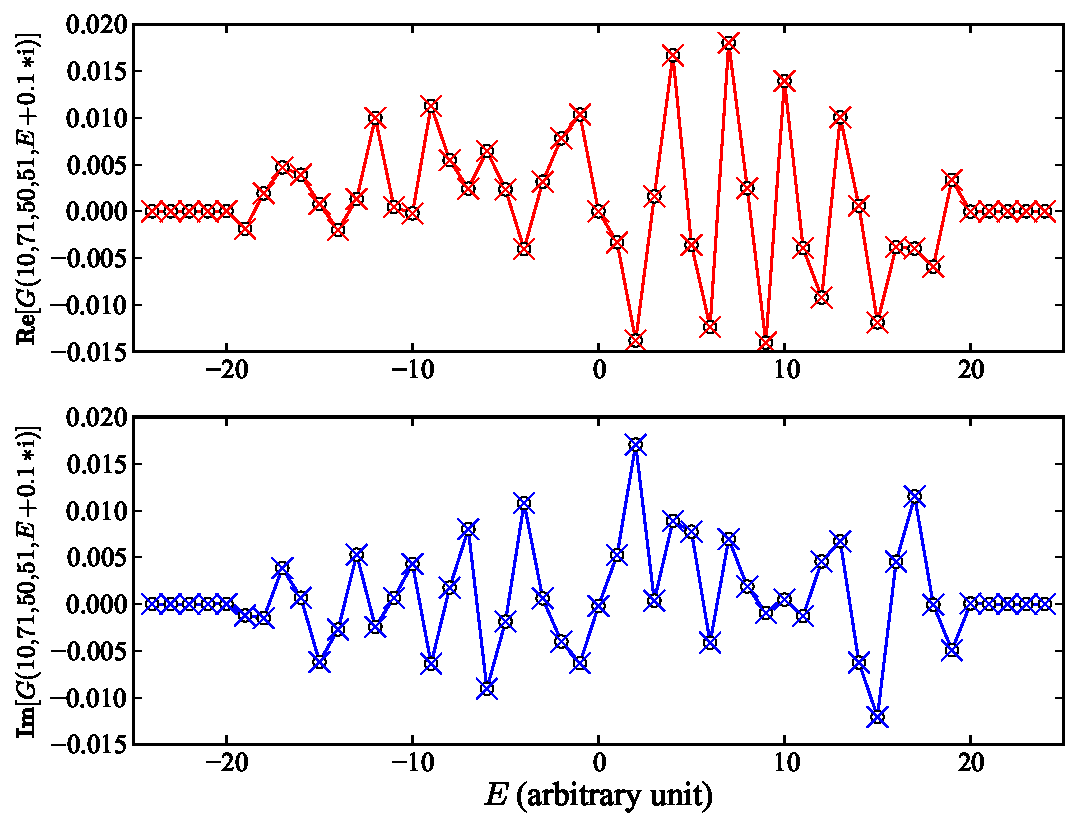
\includegraphics[width=\linewidth] {compare_GF_ordered.pdf}
\caption{ Green's function $G(10, 71, 50, 51, E + i\eta)$ with $\eta = 0.1$ as a function of energy $E$. The calculation 
was done for a finite ordered 1D crystal of 101 lattice sites with the nearest-neighbor approximation. The 
energies of the particles $e_n $ were set to zero,  and the dynamic interaction and the hopping interaction were set to $5$. The upper panel
shows the real part of the Green's function and the lower panel shows the imaginary part. The results calculated by the brute-force method
are marked with empty circles while the results obtained by our recursive method are marked by ``X''. This figure
clearly demonstrates that the recursive method produces the same results as the brute-force method. 
}
\label{fig:comparisonOrdered}
}

\addfigure{
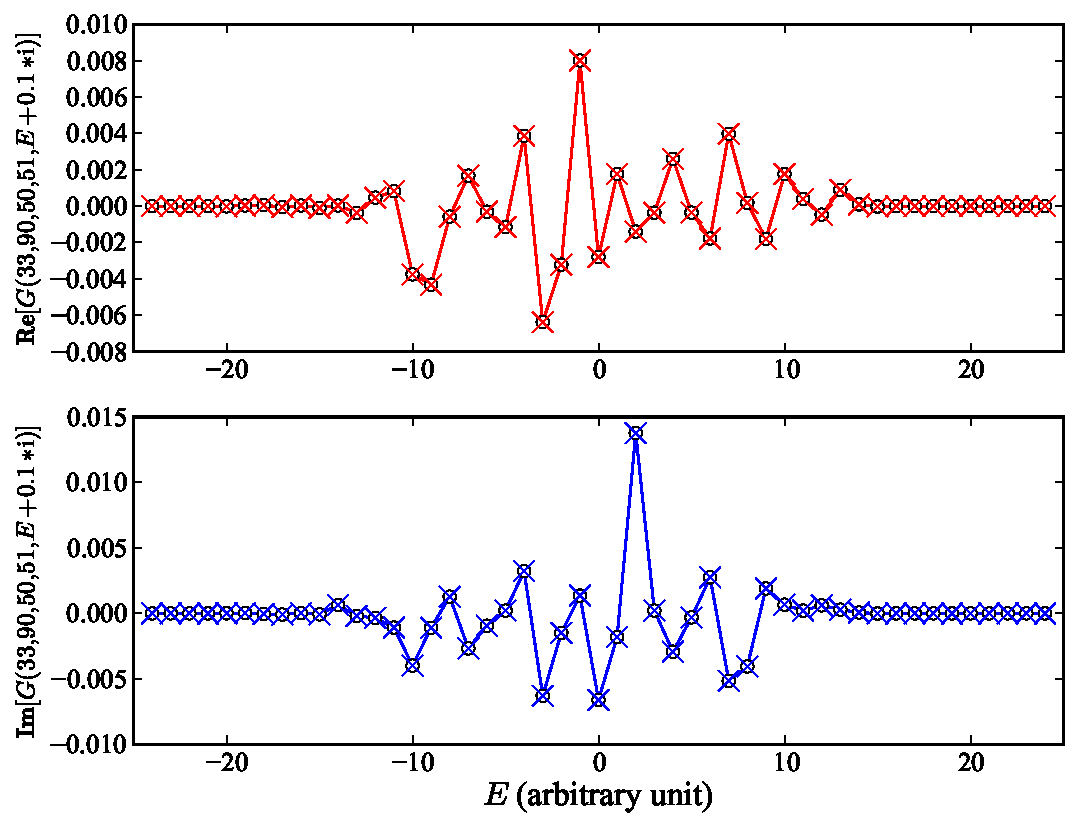
\includegraphics[width=\linewidth] {compare_GF_disordered.pdf}
\caption{ Green's function $G(33, 90, 50, 51, E + i\eta)$ with $\eta = 0.1$ as a function of energy $E$. The calculation 
was done for a finite disordered 1D crystal of 101 lattice sites with the nearest-neighbor approximation. The 
dynamic interaction and the hopping interaction were set to $5$, and allow the energies of the particles $e_n$ to fluctuate
in range $[-5, 5]$ randomly. The upper panel
shows the real part of the Green's function and the lower panel shows the imaginary part. The results calculated by the brute-force method
are marked with empty circles while the results obtained by our recursive method are marked by ``X''. This figure
clearly demonstrates that the recursive method produces the same results as the brute-force method. 
}
\label{fig:comparisonDisordered}
}

The brute-force approach is not often used in computations. Instead, the recursion method developed by Haydock 
\cite{haydock1972, haydock1975} is most widely used. For comparison purpose, we give a very brief description of the
method and compare it with our method.  The main idea of Haydock's method is to generate a series of orthonormal
vectors $\ket{u_0}$, $\ket{u_1}$, $\ket{u_2}$, $\cdots$ from the iterations
\oneline{
H \ket{u_n} = b_{n}^{*} \ket{ u_{n-1}} + a_{n} \ket{ u_{n}} + b_{n+1} \ket{ u_{n+1}} \ , \label{eqn:haydockRecursion}
}
and calculate the values of $a_n$ and $b_n$ until convergence. 
Because the Hamiltonian matrix is tridiagonal in this basis, the Green's functions can be expressed in 
term of $a_n$ and $b_n$ as
\oneline{
\bra{u_0} \hat{G}(z) \ket{u_0} = \frac{1}{z - a_0 - \frac{| b_1 |^2}{z - a_1 - \cdots } } \ .
}
For a tight-binding model with only nearest-neighbor 
interactions, the vectors $\ket{u_n}$ are a linear combinations of local states $\ket{\mathbf{R}}$ with particles residing at 
$\mathbf{R}$. The Hamiltonian has the following useful feature:
\oneline{
H \ket{\mathbf{R}} = \mathbf{t}_{\mathbf{R}, \mathbf{R-1}} \ket{ \mathbf{R-1}} + h_{\mathbf{R}, \mathbf{R}}  \ket{ \mathbf{R}} + \mathbf{t}_{\mathbf{R}, \mathbf{R+1}}  \ket{ \mathbf{R+1}} \ , \label{eqn:propertyLocalState}
}
where $h_{\mathbf{R}, \mathbf{R}}$ is the on-site energy, $\mathbf{t}$ are the matrices related to the hopping terms, and 
$\ket{ \mathbf{R-1}}$ and $\ket{ \mathbf{R+1}}$ denote the states whose particle 
positions are 1 site  different from that of $\ket{ \mathbf{R}}$. As a specific example, 
\autoref{eqn:hamOn2particleState} clearly demonstrates this property of the local state $\ket{ \mathbf{R}} = 
\ket{n}\ket{m}$. As a result of \autoref{eqn:propertyLocalState}, to calculate $G(\mathbf{R}, \mathbf{R}; z)$, 
we can initiate the recursion by setting $\ket{u_0} = \ket{\mathbf{R}}$ and $b_0 = 0$. Assuming orthonormality of 
local states, $a_0$ can be obtained by taking the product of $\bra{u_0}$ with \autoref{eqn:haydockRecursion},
\oneline{
a_0 =\bra{u_0} H \ket{u_0} = h_{\mathbf{R}, \mathbf{R}}  \ .
}
Comparing \autoref{eqn:haydockRecursion} with \autoref{eqn:propertyLocalState}, we can easily see that 
 $\ket{u_1}$ is a superposition of $\ket{ \mathbf{R-1}}$ and $\ket{ \mathbf{R+1}}$ and $b_1$ can be 
computed by requiring $\ket{u_1}$ to be normalized. To continue the recursion, we take
$n=1$ in \autoref{eqn:haydockRecursion} to obtain
\oneline{
H \ket{u_1} = b_{1}^{*} \ket{ u_{0}} + a_{1} \ket{ u_{1}} + b_{2} \ket{ u_{2}} \label{eqn:u1} \ ,
}
and let $H$ operate on $\ket{u_1}$, a superposition of  
$\ket{ \mathbf{R-1}}$ and $\ket{ \mathbf{R+1}}$, according to
 \autoref{eqn:propertyLocalState}, which gives rise to a linear combination of $\ket{ \mathbf{R-2}}$, 
$\ket{ \mathbf{R-1}}$, $\ket{ \mathbf{R}}$, $\ket{ \mathbf{R+1}}$ and $\ket{ \mathbf{R-2}}$ on the left hand side
 of \autoref{eqn:u1}. Now it is clear that $\ket{u_2}$ will also be a superposition of $\ket{ \mathbf{R-2}}$, 
$\ket{ \mathbf{R-1}}$, $\ket{ \mathbf{R}}$, $\ket{ \mathbf{R+1}}$ and $\ket{ \mathbf{R-2}}$, and $b_2$ can be
calculated from the normalization condition of $\ket{u_2}$. Follow the above analysis, we conclude that 
$\ket{u_n}$ is a superposition of these local states: $\ket{ \mathbf{R-n}}$, 
$\ket{ \mathbf{R-n+1}}$, $\cdots$, $\ket{ \mathbf{R+n-1}}$ and $\ket{ \mathbf{R+n}}$, which are within $n$-sites
distance from $\mathbf{R}$. 

Haydock's method and our method both rely on recursive calculations, but they differ a lot in numerical efficiency. 
Consider the calculation of the two-particle Green's function as an example.  If Haydock's 
method terminates the recursion at step $N$, it has to deal with vectors of size up to $\sim N^2$. 
To employ 
the same number of local states as in Haydock's method, our method sets $\mathbf{A}_{2N+1}=0$ and
 $\mathbf{\Tilde{A} }_{1}=0$, and the largest size of the vectors is about $N$, which is much smaller. Therefore
our method involves much smaller matrices and can handle much larger crystal sizes. 




\section{Application to the problem of biexciton scattering}
\label{sec:biexcitonScattering}

As a powerful analytical tool, Green's functions are often used to develop analytical formulations for  all sorts of physical 
problems. 
However, due to difficulties in their numerical computation, 
these formulations often become something of  theoretical merit only, and are rarely used for computations. For example, as will be shown below, the Green's function formulation of scattering theory is quite general and 
elegant. It 
can handle all types of scattering potentials and treat  single-particle scattering and multiple-particle scattering in the
 same way. But still the Green's functions are not used very often in scattering problems because of the numerical difficulties
 involved in their calculation\cite{Berciu2010}.  Using the new recursive
 method in \autoref{sec:recursiveGreen}, which makes the calculation easier,  the Green's
 function formulation of scattering will be used to develop a numerical method to calculate the tunneling of a biexciton state through 
 disorder potentials. This method is numerically efficient and can handle multiple impurities. 

We consider a periodic lattice with hopping interactions and dynamic interactions. Although 
the lattice is regular, disorders can still appear due to different on-site energies and different coupling strengths at 
different sites. 
We write the Hamiltonian in two parts, 
\multiline{
\hat{H} = \hat{H}_0 + \hat{H}_1 \ , \label{eqn:totalH}
}
where $\hat{H}_0$ represents an ordered array and is given by
\oneline{
\hat{H}_0 = E_0 \sum_{n} \hat{P}_n^\dag
\hat{P}_n +  \sum_{n,m \neq n}
J_{n, m}\hat{P}_n^\dag \hat{P}_m +  \frac{1}{2} \sum_{n,m \neq n} D_{n, m}
\hat{P}_{n}^\dag \hat{P}_{m}^\dag \hat{P}_{n} \hat{P}_{m} \ , \label{eqn:biexcitonHam}
} 
and $\hat{H}_1$ describes the disorders and is given by
\multiline{
\hat{H}_1 &=& \sum_{i \in S_0 } (E_i - E_0 ) \hat{P}_i^\dag
\hat{P}_i +  \sum_{\substack{i, j \neq i \\ (i, j) \in S_J } }
\left( J^{\prime}_{i, j} - J_{i, j}\right)\hat{P}_i^\dag \hat{P}_j   \nonumber \\
&+&  \frac{1}{2} \sum_{\substack{i, j \neq i \\( i, j) \in S_D }} \left( D^{\prime}_{i,j} - D_{i, j}\right)
\hat{P}_{i}^\dag \hat{P}_{j}^\dag \hat{P}_{i} \hat{P}_{j} \ , \label{eqn:disorderTerms}
} 
where $S_0$ is the set of sites whose energies are different from $E_0$, $S_J$ is the set of pairs of sites whose 
hopping terms 
$J^{\prime}$ are different from $J$, and $S_D$ is the set of pairs of sites whose dynamic interactions 
$D^{\prime}$ are different from $D$. 
%For later discussion, we define $S_{\rm disorder}$ as the set of lattice sites that
%are involved in \autoref{eqn:disorderTerms}. 
As shown in \Autoref{ch:biexciton}, if the dynamical interaction is 2 times larger than the hopping interaction,  $H_0$
will have a set of states with energies that are located outside the spectrum of two free exciton pairs. These states
are correlated  states of two excitations and are called biexcitons. The presence of $H_1$ in the Hamiltonian causes 
the eigenstates to be different from the free-biexciton state.

We are interested in the scattering of a biexciton state through disorder. For convenience, the disorder is assumed
to appear at the center region of the lattice.  The starting state is a biexciton state $\ket{\phi(K)}$ which is an 
eigenstate of $\hat{H}_0$,
\oneline{
\hat{H}_0 \ket{\phi(K)} = E(K) \ket{\phi(K)} \ .
}
 If the scattering process is elastic, we want to obtain a solution to the
full-Hamiltonian Schr\"odinger equation with the same energy as the initial biexciton state
\oneline{
(\hat{H}_0 + \hat{H}_1)\ket{\psi} = E(K) \ket{\psi} \ .
}
It can be shown that the desired solution might be
\oneline{
\ket{\psi} = \frac{1}{E(K) - \hat{H}_0} \hat{H}_1 \ket{\psi} + \ket{\phi(K)} \ .
}
There is a problem with the above solution: the operator $\frac{1}{E(K) - \hat{H}_0}$ will generate singular results
because $E(K)$ is an eigenenergy of $\hat{H}_0$. To resolve this complications, we can make the energy 
complex and the solution is then given by
\oneline{
\ket{\psi^{\pm}} = \frac{1}{E(K)\pm i\eta  - \hat{H}_0} \hat{H}_1 \ket{\psi^{\pm} } + \ket{\phi(K)}  \ . \label{eqn:lippmann-schwinger} \ ,
}
where $\eta$ is an infinitesimal positive number. 
The above equation is the Lippmann-Schwinger equation\cite{sakurai-book}. $\ket{\psi^{+}}$ and $\ket{\psi^{-}}$ are outgoing and
incoming solutions, respectively. In most cases, only $\ket{\psi^{+}}$ is interesting because it corresponds to the 
measurement at a position far away from the scatterers. Based on the definition of Green's function, 
\autoref{eqn:lippmann-schwinger} can also be written as 
\oneline{
\ket{\psi^{+}} = \ket{\phi(K)}  + \hat{G}_{0}(E(K)+ i\eta) \hat{H}_1 \ket{\psi^{\pm} } \ . \label{eqn:lippmann-schwinger-Green}
}
Substituting \autoref{eqn:lippmann-schwinger-Green} into itself and iterating gives
\oneline{
\ket{\psi^{+}} = \ket{\phi}  + \hat{G}_0^{+}  \hat{H}_1 \ket{\phi} + \hat{G}_0^{+}  \hat{H}_1 \hat{G}_0^{+}  \hat{H}_1 \ket{\phi} + \cdots \ , \label{eqn:scatteringStateInSeries}
}
where %$\hat{G}_0^{+}$ is defined by
\oneline{
\hat{G}_0^{+}(E) = \hat{G}_0 (E + i\eta) \ .
}
Based on \autoref{eqn:totalH}, we can express the Green's operator $\hat{G}$ for the total Hamiltonian in terms of
$\hat{G}_0$ and $H_1$. The derivation is presented as follows:
\multiline{
\hat{G}(z) &=& (z - \hat{H}_0 - \hat{H}_1)^{-1} \nonumber \\
&=& \bigg\{ (z- \hat{H}_0 ) \left[ 1 - (z - \hat{H}_0)^{-1} \hat{H}_1 \right] \bigg\}^{-1} \nonumber \\
&=& \left[ 1 - (z - \hat{H}_0)^{-1} \hat{H}_1 \right]^{-1} (z- \hat{H}_0 )^{-1} \nonumber \\
&=& \left[ 1 - \hat{G}_0(z) \hat{H}_1 \right]^{-1}  \hat{G}_0(z) \nonumber \\
&=&  \left[ 1 + \hat{G}_0(z) \hat{H}_1  + \hat{G}_0(z) \hat{H}_1 \hat{G}_0(z) \hat{H}_1  + \cdots \right]  \hat{G}_0(z) \nonumber \\
&=& \hat{G}_0(z) + \hat{G}_0(z) \hat{H}_1 \hat{G}_0(z) + \hat{G}_0(z) \hat{H}_1 \hat{G}_0(z) \hat{H}_1 \hat{G}_0(z) + \cdots \ . \label{eqn:Gexpansion}
}
Substituting \autoref{eqn:Gexpansion} into \autoref{eqn:scatteringStateInSeries} gives
\oneline{
\ket{\psi^{+}} = \ket{\phi}  + \hat{G}(E(K)+ i\eta) \hat{H}_1 \ket{\phi } \ . \label{eqn:scatteringState}
}
This is the equation that can be used in numerical calculations given the initial state $\ket{\phi}$ and the Green's 
function $G(z)$. 

Based on the wavefunction of a biexciton state, \autoref{eqn:biexcitonWavefunction}, derived in 
\autoref{sec:biexcitonWavefunction}, we may write the biexciton state in the two-particle basis set as
\multiline{
| \phi(K) \rangle &=& \sum\limits_{n,m \neq n} e^{iK(n+m)/2}
f_{K}(|n-m|)  \hat P_n^\dag \hat P_m^\dag \ket{0} \nonumber \\
&=& \sum\limits_{n,m \neq n} e^{iK(n+m)/2}
f_{K}(|n-m|) \ket{n, m} \ ,
}
where $f_{K}(|n-m|)$ is a function that decreases fast with increasing $|n-m|$. 
%To avoid double counting, we assume $n<m$. 
In principle, all possible two-particle states $\ket{n, m}$ with $n \neq m$ should be 
used to represent the biexciton state, but for practical purposes 
a cutoff distance $L$ for $|n-m|$ is used to greatly reduce the number of basis sets. This will hardly affect the final result
as long as  $f_{K}(|n-m|)$ decays fast enough such that $f_{K}(L) \approx 0$. In this case the biexciton state can be
rewritten as
\oneline{
| \phi(K) \rangle \approx \sum_{n}\sum_{m=n \pm 1}^{n \pm L} e^{iK(n+m)/2}
f_{K}(|n-m|) \ket{n, m} \ . \label{eqn:biexcitonSmallBasis}
}
Because the two-particle states in \autoref{eqn:biexcitonSmallBasis} can effectively represent a biexciton state, they 
are called the biexciton basis and denoted by $S_{\rm biexciton}$. 

To calculate the scattering state from \autoref{eqn:scatteringState}, let's analyze $\hat{H}_1 \ket{\phi }$ first. 
Expanding the disorder term in a two-particle basis set gives
\multiline{
\hat{H}_1 &=& \sum_{i \in S_0 } \sum_{j \neq i} (E_i - E_0 ) \ket{i, j}  \bra{i, j} +  \sum_{\substack{i, j \neq i \\ (i, j) \in S_J } }
\sum_{l\neq i, j} \left( J^{\prime}_{i, j} - J_{i, j}\right) \ket{j, l}  \bra{i, l}  \nonumber \\
&+&  \frac{1}{2} \sum_{\substack{i, j \neq i \\( i, j) \in S_D }} \left( D^{\prime}_{i,j} - D_{i, j}\right)
\ket{i, j}  \bra{i, j}  \ . \label{eqn:disorderTermsExpansion}
} 
The above equation can be derived by inserting the identity relation $\sum_{i} \ket{i}\bra{i} = I$ into the first and 
second terms of \autoref{eqn:disorderTerms}. Suppose the hopping disorder and the dynamic disorder only appear
between two sites that are within the cutoff distance $L$, we can easily see that in 
\autoref{eqn:disorderTermsExpansion} only  the two-particle states $\ket{n, m}$ with $|n-m|\leq L$ will play a role, by letting $\hat{H}_1$ operate on 
\autoref{eqn:biexcitonSmallBasis}. Since only these two-particle states are needed to represent the effective
 disorder the biexciton experiences, we call them the disorder basis $S_{\rm disorder}$. In the case of a small 
number of disorder sites, $S_{\rm disorder}$ is a small subset of $S_{\rm biexciton}$ by construction. Thus 
$\hat{H}_1 \ket{\phi }$ gives rise to a new wavefunction 
\multiline{
\ket{\phi_{\hat{H}_1}} = \hat{H}_1 \ket{\phi } = \sum\limits_{(i, j) \in S_{\rm biexciton} } c(i, j) \ket{i, j} \ ,
\label{eqn:phiH1}
}
where $ c(i, j)$ can be nonzero only if  $(i, j) \in S_{\rm disorder} $. Given
 $\ket{\phi_{\hat{H}_1}}$, we can continue to calculate the scattering state according to 
\autoref{eqn:scatteringState}. Since only a small number of coefficients $c(i, j)$ is nonzero in \autoref{eqn:phiH1}, 
 only  a small portion of the matrix that represents the Green's operator 
$\hat{G}(E(K) + i\eta)$ is needed, that is, the matrix elements $\bra{i^{\prime}, j^{\prime}}\hat{G}(E(K) + i\eta) \ket{i, j}$ 
with $\ket{i, j}$ being states in the disorder basis. This task can be efficiently handled by the recursive method in
\autoref{sec:recursiveGreen} by setting the initial particle positions $(n^{\prime}, m^{\prime})$ to be every site 
pairs $(i, j)$ in $S_{\rm disorder}$. 

To prevent the processes of a biexciton breaking into two free excitons, we assume the dynamic interaction is more
than 2 times larger than the hopping interaction such that the energy of a biexciton is well separated from the 
energy spectrum of two free excitons. 
During the scattering process, the energy must be conserved, and thus the
scattering wavefunction has the following asymptotic behavior
\multiline{
 \ket{\psi} \rightarrow \left\{ 
  \begin{array}{l l}
    \ket{\phi(K)} + \mathbf{R}\ket{\phi(-K)} & \quad \text{for $n, m \rightarrow -\infty $}\\
    \mathbf{T}\ket{\phi(K)} & \quad \text{for $n, m \rightarrow \infty $}
  \end{array} \right. \ , \label{eqn:scatteringAsymptotic}
}
if the initial biexciton state $\ket{\phi(K)}$ incidents from the left with its eigenenergy $E(K)$. 
This asymptotic behavior can be used to calculate the transmission coefficient of a biexciton through disorder. 
In principle, scattering calculations usually assume a infinitely large space, but in practice, a finite crystal  
with sufficiently large size is used. We start the calculation from an initial biexciton state $\phi(K)$ with
eigenenergy $E(K)$, and then calculate the scattering state $\ket{\psi}$ using \autoref{eqn:scatteringState}. 
The transmission coefficient can then be deduced from \autoref{eqn:scatteringAsymptotic} by choosing two sites
$n$ and $m$ to the far right of the disorder region, that is
\oneline{
t = \frac{ \langle{n, m} \ket{\psi} } { \langle{n, m} \ket{\phi(K)} } \ .
}
Note that the scattering wavefunction $\ket{\psi}$ must be properly normalized with respect to the finite crystal. 

\section{Summary}
\label{sec:summaryGreenFunc}

In this chapter, a recursive method to calculate lattice Green's functions is described. The essential idea 
is to group Green's functions into different sets of vectors and rewrite the equation of motion of Green's function as a 
recursion relation linking three consecutive vectors. Based on physical reasoning, certain vectors are 
assumed to be zero and then substituted into the corresponding recursion relations to express one set
of Green's function in terms of another set of Green's function. By iterating on the recursion relation, a 
chain of relationships between each two consecutive vectors can be obtained. Finally, the vector at the end of this 
relationship chain can be calculated by solving a linear equation, and all the vectors can be calculated one by one
through the relationship chain.   
The method can handle a system with arbitrary 
disorder, and can be easily extended to systems with interactions of longer (but finite) range, and to systems with
high dimensionality. To show the numerical efficiency of the method, it was compared with the brute-force method and
 Haydock's method.  Our method involves vectors of much smaller sizes. As an 
application, we described using the recursive method to calculate the Green's functions  to study the 
scattering of a biexciton state by impurities. 
 
